

\tikzset{every picture/.style={line width=0.75pt}} %set default line width to 0.75pt        

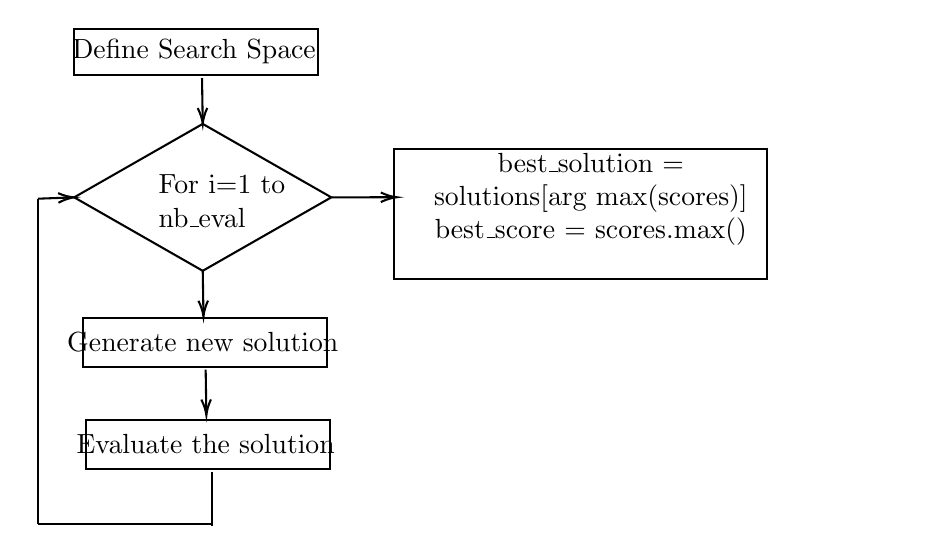
\begin{tikzpicture}[x=0.75pt,y=0.75pt,yscale=-1,xscale=1,scale=0.70]
%uncomment if require: \path (0,450); %set diagram left start at 0, and has height of 450

%Shape: Rectangle [id:dp287484076214092] 
\draw   (56,47.5) -- (224,47.5) -- (224,79.5) -- (56,79.5) -- cycle ;

%Flowchart: Decision [id:dp7221416464500721] 
\draw   (144.5,113) -- (233,163.57) -- (144.5,214.14) -- (56,163.57) -- cycle ;
%Shape: Rectangle [id:dp2168629735514297] 
\draw   (62,246.5) -- (230,246.5) -- (230,280.5) -- (62,280.5) -- cycle ;

%Shape: Rectangle [id:dp9454846930994444] 
\draw   (64,316.5) -- (232,316.5) -- (232,350.5) -- (64,350.5) -- cycle ;

%Straight Lines [id:da990417600494777] 
\draw    (144,81.5) -- (144.47,111) ;
\draw [shift={(144.5,113)}, rotate = 269.09] [color={rgb, 255:red, 0; green, 0; blue, 0 }  ][line width=0.75]    (10.93,-3.29) .. controls (6.95,-1.4) and (3.31,-0.3) .. (0,0) .. controls (3.31,0.3) and (6.95,1.4) .. (10.93,3.29)   ;
%Straight Lines [id:da6691446751134834] 
\draw    (144.5,214.14) -- (144.73,228.47) -- (144.97,243.64) ;
\draw [shift={(145,245.64)}, rotate = 269.09] [color={rgb, 255:red, 0; green, 0; blue, 0 }  ][line width=0.75]    (10.93,-3.29) .. controls (6.95,-1.4) and (3.31,-0.3) .. (0,0) .. controls (3.31,0.3) and (6.95,1.4) .. (10.93,3.29)   ;
%Straight Lines [id:da7532189586068166] 
\draw    (146.5,282.14) -- (146.97,311.64) ;
\draw [shift={(147,313.64)}, rotate = 269.09] [color={rgb, 255:red, 0; green, 0; blue, 0 }  ][line width=0.75]    (10.93,-3.29) .. controls (6.95,-1.4) and (3.31,-0.3) .. (0,0) .. controls (3.31,0.3) and (6.95,1.4) .. (10.93,3.29)   ;
%Straight Lines [id:da9977767621146708] 
\draw    (151,352.5) -- (151,389.5) ;
%Straight Lines [id:da46977265796894596] 
\draw    (151,388.5) -- (31,388.5) ;
%Straight Lines [id:da26924168681760574] 
\draw    (31,164.5) -- (31,388.5) ;
%Straight Lines [id:da07884456987557487] 
\draw    (31,164.5) -- (54,163.65) ;
\draw [shift={(56,163.57)}, rotate = 177.87] [color={rgb, 255:red, 0; green, 0; blue, 0 }  ][line width=0.75]    (10.93,-3.29) .. controls (6.95,-1.4) and (3.31,-0.3) .. (0,0) .. controls (3.31,0.3) and (6.95,1.4) .. (10.93,3.29)   ;
%Straight Lines [id:da06791709888118524] 
\draw    (233,163.57) -- (276,163.5) ;
\draw [shift={(278,163.5)}, rotate = 179.91] [color={rgb, 255:red, 0; green, 0; blue, 0 }  ][line width=0.75]    (10.93,-3.29) .. controls (6.95,-1.4) and (3.31,-0.3) .. (0,0) .. controls (3.31,0.3) and (6.95,1.4) .. (10.93,3.29)   ;
%Shape: Rectangle [id:dp7667361145975681] 
\draw   (275.87,130) -- (533,130) -- (533,220) -- (275.87,220) -- cycle ;


% Text Node
\draw (138.5,63.37) node   [align=left] {\begin{minipage}[lt]{113.56pt}\setlength\topsep{0pt}
\begin{center}
Define Search Space
\end{center}

\end{minipage}};
% Text Node
\draw (112,146) node [anchor=north west][inner sep=0.75pt]   [align=left] {For i=1 to\\nb\_eval};
% Text Node
\draw (144.5,263.36) node   [align=left] {\begin{minipage}[lt]{113.56pt}\setlength\topsep{0pt}
\begin{center}
Generate new solution
\end{center}

\end{minipage}};
% Text Node
\draw (146.5,333.36) node   [align=left] {\begin{minipage}[lt]{113.56pt}\setlength\topsep{0pt}
\begin{center}
Evaluate the solution
\end{center}

\end{minipage}};
% Text Node
\draw (411.61,164.77) node   [align=left] {\begin{minipage}[lt]{214.36pt}\setlength\topsep{0pt}
\begin{center}
best\_solution = \\solutions[arg max(scores)]\\best\_score = scores.max()
\end{center}

\end{minipage}};


\end{tikzpicture}
